%% LyX 2.3.6 created this file.  For more info, see http://www.lyx.org/.
%% Do not edit unless you really know what you are doing.


\documentclass[10pt]{article}
\usepackage{helvet}
\usepackage{caption}
\usepackage{float}
\usepackage{xcolor}
\usepackage[framemethod=TikZ]{mdframed}
\renewcommand{\familydefault}{\sfdefault}
\usepackage[T1]{fontenc}
\usepackage[utf8]{inputenc}
\usepackage[a4paper]{geometry}
% \geometry{verbose,tmargin=5cm,bmargin=4cm,lmargin=5cm,rmargin=5cm}
\usepackage{fancyhdr}
\pagestyle{fancy}
\setlength{\parskip}{6pt}
\setlength{\parindent}{0pt}
\usepackage{tcolorbox}
\usepackage{amsmath}
\usepackage{amsthm}
\usepackage{amssymb}
\usepackage{todonotes}
\usepackage{graphicx}
\usepackage[backend=bibtex,maxbibnames=99]{biblatex}
\addbibresource{main.bib}

\floatstyle{plaintop}
\newfloat{listing}{htbp}{lop}
\floatname{listing}{Listing}

\definecolor{lightgray}{gray}{0.9} % Defines the color 'lightgray' with a specific shade.

\newmdenv[
  linecolor=lightgray,
  backgroundcolor=white,
  outerlinewidth=1pt,
  roundcorner=2pt,
  innertopmargin=10pt,
  innerbottommargin=10pt,
  innerrightmargin=10pt,
  innerleftmargin=10pt
]{greyborder}


\makeatletter

\DeclareMathOperator*{\argmin}{arg\,min}
\DeclareMathOperator*{\del}{\nabla}

%%%%%%%%%%%%%%%%%%%%%%%%%%%%%% LyX specific LaTeX commands.
%% A simple dot to overcome graphicx limitations
\newcommand{\lyxdot}{.}

%%%%%%%%%%%%%%%%%%%%%%%%%%%%%% User specified LaTeX commands.
\usepackage{tcolorbox}
\usepackage{amsthm}
\usepackage{lastpage}
\usepackage{fancyhdr}
\usepackage{accents}
\usepackage{titlesec}
\usepackage{marginnote}
% \titleformat{\section}[block]{\normalfont\bfseries}{}{0em}{}


\usepackage{enumitem}
\usepackage{comment}
% \setlist{nolistsep}

\usepackage{tcolorbox}
\definecolor{light-blue}{cmyk}{0.24, 0.12, 0.0, 0.04, 1.00}
% \titlespacing\section{0pt}{0pt}{0pt}
% \titlespacing\subsection{0pt}{0pt}{0pt}
% \titlespacing\subsubsection{0pt}{0pt}{0pt}

\setlength{\headheight}{40pt}

\makeatother

\title{Week 2 Optimisation for Machine Learning}
\author{Neimhin Robinson Gunning, 16321701}
\date{\today}

\begin{document}
\maketitle
\lhead{Neimhin Robinson Gunning} \rhead{CS7CS4 Week 2 Assignment}


\begin{figure}
  \begin{center}
    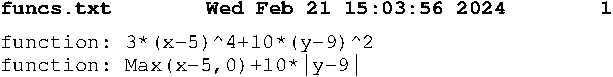
\includegraphics[width=0.95\textwidth]{funcs.pdf}
  \end{center}
  \caption{Two bivariate functions downloaded from \texttt{https://www.scss.tcd.ie/Doug.Leith/CS7DS2/week4.php}}\label{lst:funcs.txt}
\end{figure}


Let \begin{equation}
  f(x,y)=3(x-5)^4+10(y-9)^2
  \label{eq:f}
\end{equation}
and 
\begin{equation}
  g(x,y)=\max(x-5,0)+10|y-9|
  \label{eq:g}
\end{equation}

Using \texttt{sympy} we find the derivatives:
$$\nabla f=[\frac{df}{dx},\frac{df}{dy}]=[12(x-5)^{3},20y-180]$$
$$\nabla g=[\frac{dg}{dx},\frac{dg}{dy}]=[\text{Heaviside}(x-5),10\text{sign}(y-9)]$$


Clearly, the minimum of $f(x,y)$ is $0$ and they is minimized by $x=5$, $y=9$.
The other function $g(x,y)$ also has minimum $0$ but is minized by any of $x\in[-\infty,5]$ and $y=9$.

The Polyak step size is \begin{equation}
  \alpha_{\text{Polyak}}=\frac{f(x)-f^*}{\del f(x)^T\del f(x)}
  \label{eq:polyak-step}
\end{equation}
where $x$ is the parameter vector, $f(x)$ is the function to optimise, and $f^*\approx\min_xf(x)$.

\begin{figure}
  \begin{center}
    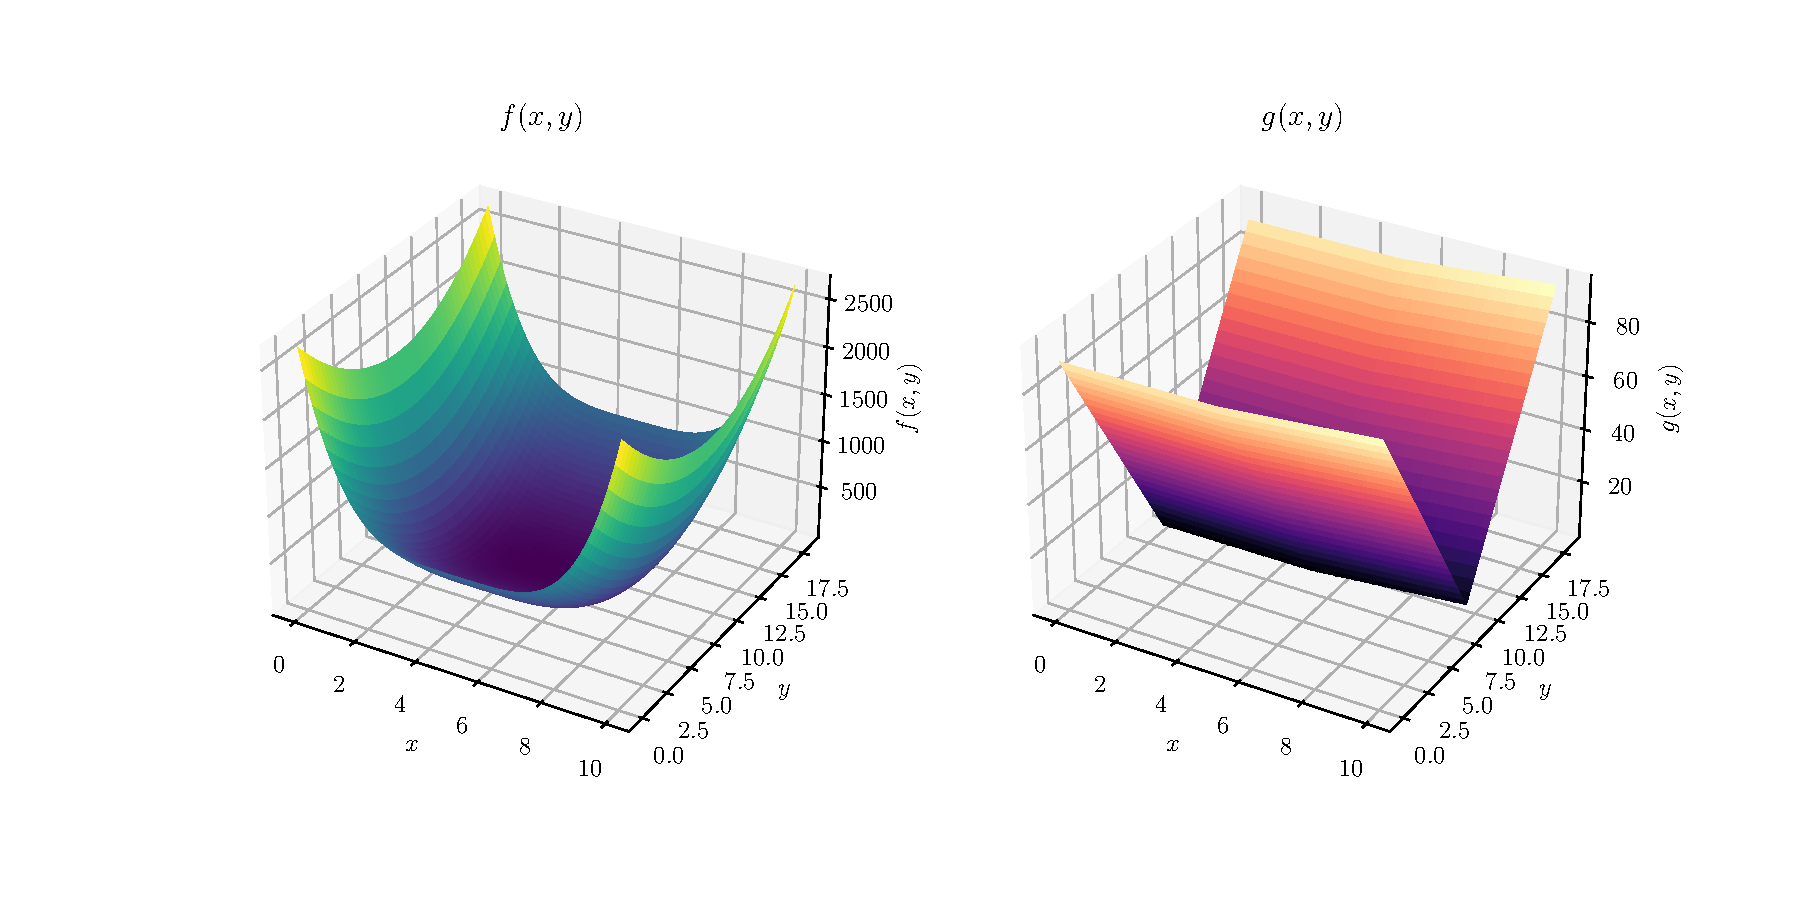
\includegraphics[width=0.95\textwidth]{fig/f-g.pdf}
  \end{center}
  \caption{}\label{fig:f-and-g}
\end{figure}

\begin{listing}
  \includegraphics[width=0.95\textwidth]{tmp/polyak_step_size.pdf}
  \caption{A python function to calculate the Polyak step size on a \texttt{sympy} function.}
  \label{lst:polyak-step}
\end{listing}

\bigskip{}
\printbibliography
\end{document}
